\documentclass[brazil, 11pt]{exam}
\usepackage[brazil]{babel}
\usepackage{multicol}
\usepackage{amsmath}
\usepackage{multirow}
\usepackage{tabularx}
\usepackage{siunitx}
\usepackage{tikz}
\usepackage{xcolor}
\usepackage{tcolorbox}
\usepackage{graphicx}
\usepackage{enumitem} % Pacote para personalização de listas

% Configuração do layout da página
\usepackage[a4paper, %
            top=20mm, 
            bottom=15mm, %
            left=15mm, %
            right=15mm, %
            footskip=2mm]{geometry}%, 
            %showframe] %
            %{geometry}

% Configurando parágrafos
\setlength{\parindent}{0cm}
\setlength{\parskip}{1em}

% Configuração das colunas do documento
\setlength{\columnsep}{0.0cm}
\setlength{\columnseprule}{0.0pt}

% Alterando a fonte
\renewcommand{\familydefault}{\sfdefault}

% Gabarito automatico. Baseado em:
% https://tex.stackexchange.com/questions/574316/how-to-produce-answer-key-in-exam-class-for-multiple-choice-type-of-question
\newcommand\Answers{} % Accumulates triples {{question number}{choice number}{answer}}
\newcommand\Correct[1]{% {answer} % adds new triple to \Answers
    \xdef\Answers{\Answers{{\arabic{question}}{\Alph{choice}}{#1}}}%
    #1
}
\newcommand\printAnswer[3]{% {question number}{choice number}{answer} % format answer
    %\par\noindent #1. Ans: (#2) #3\par
    \par\noindent #1. #2\par
}
\newcommand\printAnswers{% do \printAnswer for every answer in \Answers
    \expandafter\printAnswersX\Answers{}%
}
\newcommand\printAnswersX[1]{% {{qu. number}{ch. number}{answer}} % auxilary command implementing loop
    \def\tmp{#1}%
    \ifx\tmp\empty
        \let\tmp\relax
    \else
        \def\tmp{\printAnswer#1\printAnswersX}
    \fi
    \tmp  
}

% Numeração das páginans
\footer{}{\thepage}{}

% Unidades de medida do jeito certo
\sisetup{per-mode = symbol,
    output-decimal-marker = {,}, 
    inter-unit-product=\ensuremath{{}\cdot{}}}
\DeclareSIUnit{\rev}{rev}
\DeclareSIUnit{\volta}{voltas}
\DeclareSIUnit{\boe}{boe}
\DeclareSIUnit{\batimentos}{batimentos}

% Define a unidade da pontuação como " pt"
\pointpoints{\tiny ponto}{\tiny pontos}

% Ambiente customizado para enunciar questões
\qformat{\hspace{-1.4em}
    \tikz[baseline=(X.south)]{
        \node[minimum width=2em, 
            minimum height=3ex, 
            shape=rectangle, 
            fill=black, 
            text=white, 
            inner sep=0pt, 
            outer sep=0pt] (X) {\textbf{\thequestion}}
    }
    \hspace{-2.84em}
    \tikz[baseline=(X.south)]{
        \node[minimum width=0.85\columnwidth, 
            minimum height=3ex, 
            shape=rectangle, 
            fill=lightgray, 
            text width=0.8\columnwidth,
            align=right,
            inner sep=0pt, 
            outer sep=0pt] (X) {\tiny\thepoints}
    }
    \vspace{1ex}
}

% Circulo decorativo das respostas alternativas
\newcommand*\circled[1]{\tikz[baseline=(char.base)]{
    \node[shape=circle, %
    draw, %
    inner sep=0.3pt, %
    minimum size=0.9em, %
    fill=black, %
    text=white] (char) {\textbf{\footnotesize #1}};} \ }

% Formatando letras das "opções"
\renewcommand{\choicelabel}{\circled{\alph{choice}}}

% Indentando letras das opções:
\renewcommand{\choiceshook}{%
    \setlength{\leftmargin}{0.0em}%
    \setlength{\labelwidth}{0.0em}%
    \setlength{\labelsep}{0.0em}%
    %\setlength{\labelwidth}{-\labelsep}%
    %\addtolength{\itemindent}{\labelwidth}%
}

% Ajustando alinhamento dos elementos do cabeçalho
\newcolumntype{Y}{>{\raggedright\arraybackslash}X}
\newcolumntype{Z}{>{\raggedleft\arraybackslash}X}

% Redefinindo o \maketitle para a classe exam
\makeatletter
\renewcommand{\maketitle}{%
    \noindent\hspace*{-0.4em}%
    %\begin{table}[t]
        \begin{tabularx}{\dimexpr\linewidth-0.5em}{Y Z}
            \multirow{4}{*}{
\includegraphics{logo-ifce-bat-11pt.pdf}}
            & \\
            & \curso \\
            & \noindent\atividade\ de \disciplina\\
            & \professor $ \cdot$ \periodo \\
        \end{tabularx} 
        \vspace{-2ex}
    %\end{table}
    
    \noindent\hspace*{-0.9em}
    \setlength{\fboxsep}{8pt}
    \setlength{\fboxrule}{0.25pt}
    \fbox{Estudante:\hspace{11cm} Data:\hspace{3.05cm}} 
    \vspace{1ex}
}
\makeatother

% Configuração da caixa de orientações, avisos, e gabarito de respostas
\usepackage{tcolorbox}
\tcbset{fontupper=\small,colback=white,colframe=black,boxrule=0.5pt}

% Identificação do documento 
\newcommand{\curso}{Técnico Integrado em Comércio}
\newcommand{\disciplina}{Física Complementar}
\newcommand{\atividade}{Prova}
\newcommand{\professor}{Prof. Paulo Santiago }
\newcommand{\periodo}{2025-1}

\begin{document}

\maketitle

% Início das colunas
\begin{multicols}{2}

% Quadro de orientações, avisos, e gabarito de respostas
    \begin{tcolorbox}[width=0.95\linewidth]%[width=0.9\columnwidth]
        \textbf{Orientações} \tcblower
        \begin{itemize}
            %\item A prova poderá ser feita em duplas, sem consulta e sem interação entre diferentes duplas.
            \item A prova é individual, sem consulta. Qualquer violação habilitará a invalidação da mesma. 
            \item Cada estudante deve entregar sua prova identificada com nome e data.
            \item A prova será recebida somente após 1 hora do seu início.
            %\choice As questões 01, 02, 05, 07, 08 e 09 devem estar acompanhada dos cálculos.
            \item Só serão válidas as respostas fornecidas no cartão-resposta logo abaixo. 
            \item É necessário fornecer os 3 dígitos finais da matrícula para devida identificação.
            \item Use caneta azul ou preta para preencher o cartão-resposta.
            \item Deve-se preencher por inteiro o espaço dentro do círculo do cartão-resposta para que a questão seja válida.
            \item Não faça marcações dentro da área do cartão resposta se não for referente ás respostas ou final do número da matrícula. 
        \end{itemize}
        
        \vspace{0.5cm}
        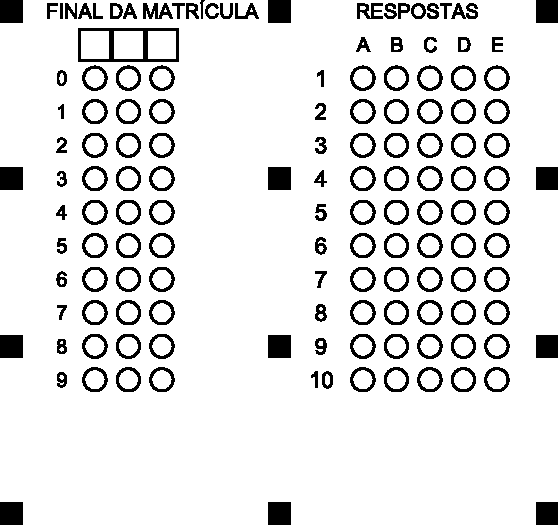
\includegraphics[width=\columnwidth,keepaspectratio]{gabarito.pdf}
        
        \vspace{0.5cm}
        
        \begin{center}
            Boa prova!
        \end{center}
    \end{tcolorbox}


\begin{questions}

\begin{question}[1] % Enem 2012 PPL
\begin{minipage}{0.93\linewidth}\vspace{1ex}
\hspace{2em} Está é uma questão de exemplo. Normalmente há um texto que pode ser acompanhado de uma figura, uma tabela, uma lista numerada, ou qualquero outra forma de apresentação da informação. 
\hspace{2em} Em seguida, são apresentadas as opções para escolha da resposta.
\begin{choices}
    \CorrectChoice\Correct{} Este é o item correto. 
    \choice Um item qualquer para ilustrar uma lista de opções.
    \choice Vamos fazer questões objetivas de 5 itens.
    \choice É possível ter uma quantidade maior de itens.
    \choice Um item para encerrar o exemplo.
\end{choices}
\end{minipage}
\end{question}

% Espaçador para final de colunas
\begin{center}
    ---------[ espaço para cálculos ]---------
\end{center}\vfill\null

% Relação de respostas certas
Respostas
\begin{multicols}{2}
    \printAnswers    
\end{multicols}


\end{questions}
\end{multicols}



\end{document}